\documentclass[10pt,a4paper]{article}
\usepackage[margin=1.25in]{geometry}
\usepackage{fancyhdr} % fancy header
\pagestyle{fancy} % so fancy
\usepackage[round]{natbib} % bibliography
\usepackage{graphicx} % for importing graphics / figures
\usepackage{booktabs} % publication-worthy tables
\usepackage{multirow}
\usepackage{adjustbox} % makes tables fit nicely on the page


\lhead{Josh MEYER}
\rhead{Dissertation Prospectus}
\cfoot{} %% make empty to get rid of the page number %% \cfoot{Page \thepage}
\renewcommand{\footrulewidth}{0.4pt} %% this puts a fancy line at the footer


\begin{document}


\section{What I'm doing \& Why it's Extremely Cool}

I'm creating Neural Nets which better classify data from unseen conditions, without any explicit adaptation of model parameters or data transformations.

My approach is extremely cool because it doesn't require tons of data, it is not specific to some dataset, and it can be used to build any Neural Net (not just for speech recognition).


\section{Overview of Speech Recognition}

This section contains an overview of the training and testing procedures for standard automatic speech recognition (ASR) pipelines. The overview will provide the reader with a technical grounding in ASR, so that the rest of the dissertation will have some point of reference. 


\begin{itemize}

\item \textbf{Gaussians + HMMs}
  
\item \textbf{Neural Nets + HMMs}
  
\item \textbf{end-to-end Neural Nets}

\end{itemize}


\section{Background Literature}

Here I will cover the literature relevant to working with small (or completely new) datasets. There are two main approaches, (1) adapt a model from one training dataset to a new, smaller dataset; (2) create a model that is robust enough to handle data from multiple domains. 

\begin{itemize}

\item \textbf{Model Adaptation: (e.g. Speaker; Language)}

      %% 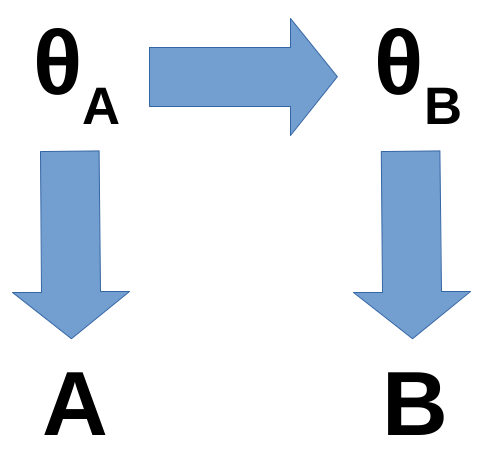
\includegraphics[width=.2\textwidth,keepaspectratio]{figs/transfer.png}
    
  
\item \textbf{Model Robustness: (e.g. Noise; Channel)}

    %% 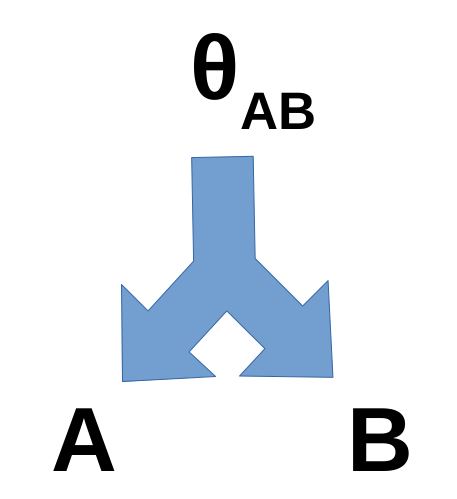
\includegraphics[width=.2\textwidth,keepaspectratio]{figs/robustness.png}
  
\end{itemize}




\section{Experiments}

This section contains the main contributions of the dissertation research.

The aim of the dissertation is to investigate training methods for acoustic modeling to be used in the Neural Net + HMM ASR pipeline.

\subsection{Data}
I aim to produce acoustic models which perform better (i.e. lower Word Error Rates) on datasets which are not similar the original training dataset.

The differences between the training and testing data will be (1) the recording noise conditions, (2) who the speaker is, or (3) what language the speaker is using.


\begin{table}[htbp]
  \centering
  \begin{adjustbox}{width=.75\textwidth}
    \begin{tabular}{clcc}
      \toprule
      && \multicolumn{2}{c}{\textsc{Corpus}}\\
      && \textbf{Train} & \textbf{Test}\\
      \midrule
      \multirow{3}{*}{\textsc{Audio Condition}} &\textbf{Noise} & TIDIGITS & Aurora 5 \\
      &\textbf{Speaker} & LibriSpeech-A & LibriSpeech-B \\
      &\textbf{Language} & LibriSpeech & Kyrgyz Audiobook \\
      \bottomrule
    \end{tabular}
    \label{table:data}
  \end{adjustbox}
  
  \caption{Speech Corpora}
  
\end{table}


\subsection{Model Training Procedure}

I investigate methods of neural net training with Multi-Task Learning (MTL).

Typically, the tasks used in MTL are assumed to exist and be useful in some other application (e.g. POS tagging as an additional task to learn dependency parsing). However, a less common approach to MTL training is to create completely new tasks.

This dissertation investigates the creation of new tasks for MTL, either using (1) linguist-expert knowledge, (2) ASR Engineer-expert knowledge, or (3) general Machine Learning knowledge.

The latter two knowledge sources are useful for buidling acoustic models, but not much else. On the other hand, the final source of knowledge (general machine learning concepts) can be applied to any classification problem.

The three knowledge sources will be abbreviated as such:
  
\begin{itemize}
\item  (\textsc{LING}) \textbf{Linguistic Knowledge} 
\item (\textsc{ASR}) \textbf{Traditional Speech Recognition Pipeline}
\item (\textsc{ML}) \textbf{General Machine Learning}
\end{itemize}


Each of these knowledge sources contains a wealth of ideas which could be used in MTL for acoustic modeling, and I will consolidate each knowledge source into three experiments. With three experiments for each knowledge source, my dissertation will contain nine (9) experimental conditions.

Specifically, I will perform the following experiments:

\begin{table}[htbp]
  \centering
  \begin{adjustbox}{width=.75\textwidth}
    \begin{tabular}{cccc}
      \toprule
      & \multicolumn{3}{c}{\textsc{Knowledge Source}}\\
      & \textbf{LING} & \textbf{ASR} & \textbf{ML}\\
      \midrule
      \multirow{3}{*}{\textsc{Experiments}} & voicing & monophones &  k-means \\
      & place & $1/2$ triphones & random forests  \\
      & manner & triphone variations &  bootstrapped resamples  \\
      \bottomrule
    \end{tabular}
    \label{table:data}
  \end{adjustbox}
  
  \caption{Experimental Setup}
  
\end{table}


When these experiments will be applied to each of the three audio conditions, we get the following:

  


\begin{table}[htbp]
  \centering
  \begin{adjustbox}{width=.95\textwidth}
    \begin{tabular}{ccclc}
      \toprule
      \textbf{Data Condition} & \textbf{Train Data} & \textbf{Test Data} & \textbf{MTL Training Tasks} & \textbf{Num. Exps} \\
      \midrule
      \multirow{4}{*}{\textsc{Noise}} & \multirow{4}{*}{\textsc{TIDIGITS}} & \multirow{4}{*}{\textsc{Aurora 5}} & Basline & 1\\
      & & & Baseline + LING & 3   \\
      & & & Baseline + ASR  & 3  \\
      & & & Baseline + ML   & 3  \\
      \midrule
      \multirow{4}{*}{\textsc{Speaker}} & \multirow{4}{*}{\textsc{LibriSpeech-A}} & \multirow{4}{*}{\textsc{LibriSpeech-B}} & Baseline & 1 \\
      & & & Baseline + LING & 3  \\
      & & & Baseline + ASR  & 3  \\
      & & & Baseline + ML   & 3  \\     \midrule
      \multirow{4}{*}{\textsc{Language}} & & \multirow{4}{*}{\textsc{Kyrgyz-B}} & Baseline & 1\\
      & \textsc{LibriSpeech +} & & Baseline + LING  & 3 \\
      &  \textsc{Kyrgyz-A} & & Baseline + ASR   & 3 \\
      & & & Baseline + ML & 3 \\
      \midrule
      &&&& 30\\
      \bottomrule\\
    \end{tabular}
    \label{table:data}
  \end{adjustbox}
  
  \caption{Experimental Setup}
  
\end{table}



\end{document}



 
